\documentclass[10pt]{article}
\usepackage[paperwidth=198mm,paperheight=59mm,margin=1mm]{geometry}
\usepackage{newtxtext,newtxmath,tikz,pgfplots}
\pgfplotsset{compat=1.18}
\definecolor{methodblue}{HTML}{216A85}
\definecolor{controlgray}{HTML}{555555}
\definecolor{accentorange}{HTML}{A64B1D}
\pagestyle{empty}
\begin{document}\noindent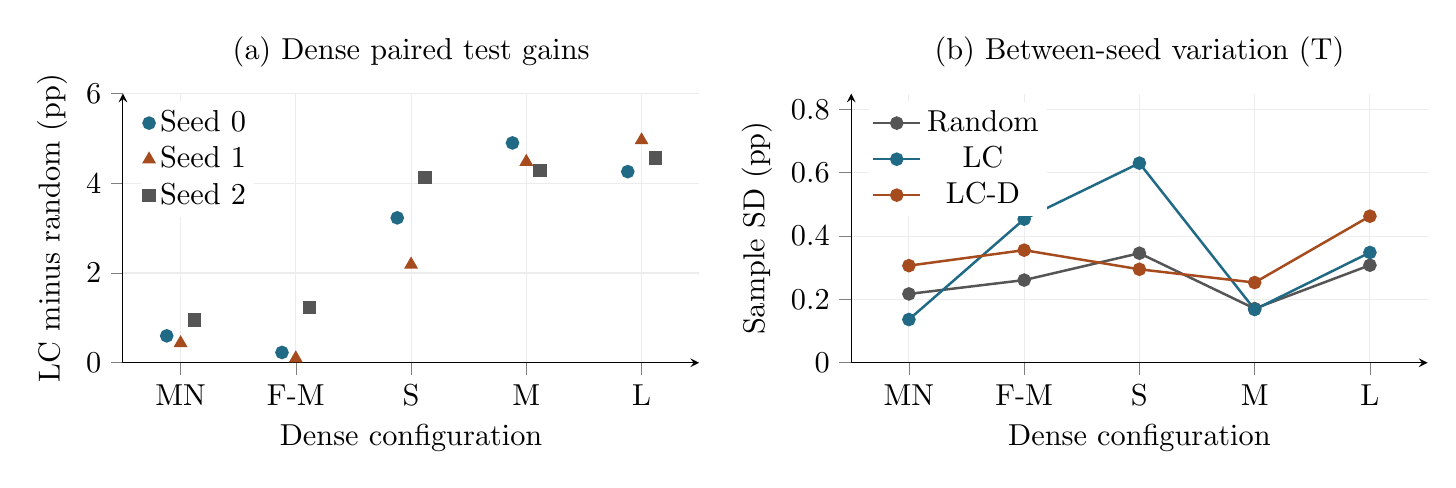
\begin{tikzpicture}
\begin{axis}[width=89mm,height=50mm,axis lines=left,tick align=outside,grid=major,grid style={gray!15},scaled ticks=false,tick label style={font=\fontsize{11}{13}\selectfont},label style={font=\fontsize{11}{13}\selectfont},title style={font=\fontsize{11}{13}\selectfont},legend style={font=\fontsize{11}{13}\selectfont,draw=none,fill=white,inner sep=1pt},title={(a) Dense paired test gains},xmin=-.5,xmax=4.5,ymin=0,ymax=6,xtick={0,1,2,3,4},xticklabels={MN,F-M,S,M,L},xlabel={Dense configuration},ylabel={LC minus random (pp)},legend pos=north west]
\addplot+[color=methodblue,mark=*,mark size=2pt,line width=0.9pt,mark options={solid,fill=methodblue,draw=methodblue},only marks] coordinates {(-0.12,0.60000026)(0.88,0.22999996)(1.88,3.2299999)(2.88,4.9000002)(3.88,4.26)};
\addlegendentry{Seed 0}
\addplot+[color=accentorange,mark=triangle*,mark size=2pt,line width=0.9pt,mark options={solid,fill=accentorange,draw=accentorange},only marks] coordinates {(0,0.43999988)(1,0.10000062)(2,2.1899998)(3,4.4800001)(4,4.9600003)};
\addlegendentry{Seed 1}
\addplot+[color=controlgray,mark=square*,mark size=2pt,line width=0.9pt,mark options={solid,fill=controlgray,draw=controlgray},only marks] coordinates {(0.12,0.94999987)(1.12,1.2300001)(2.12,4.1300001)(3.12,4.2900001)(4.12,4.5600001)};
\addlegendentry{Seed 2}
\end{axis}
\begin{axis}[width=89mm,height=50mm,axis lines=left,tick align=outside,grid=major,grid style={gray!15},scaled ticks=false,tick label style={font=\fontsize{11}{13}\selectfont},label style={font=\fontsize{11}{13}\selectfont},title style={font=\fontsize{11}{13}\selectfont},legend style={font=\fontsize{11}{13}\selectfont,draw=none,fill=white,inner sep=1pt},at={(9.25cm,0)},anchor=south west,title={(b) Between-seed variation (T)},xmin=-.5,xmax=4.5,ymin=0,ymax=.85,xtick={0,1,2,3,4},xticklabels={MN,F-M,S,M,L},xlabel={Dense configuration},ylabel={Sample SD (pp)},legend pos=north west]
\addplot+[color=controlgray,mark=*,mark size=2pt,line width=0.9pt,mark options={solid,fill=controlgray,draw=controlgray}] coordinates {(0,0.21733222)(1,0.26102353)(2,0.34588056)(3,0.17097752)(4,0.30805842)};
\addlegendentry{Random}
\addplot+[color=methodblue,mark=*,mark size=2pt,line width=0.9pt,mark options={solid,fill=methodblue,draw=methodblue}] coordinates {(0,0.13650381)(1,0.45346795)(2,0.63042328)(3,0.16802787)(4,0.34818579)};
\addlegendentry{LC}
\addplot+[color=accentorange,mark=*,mark size=2pt,line width=0.9pt,mark options={solid,fill=accentorange,draw=accentorange}] coordinates {(0,0.30664855)(1,0.3555744)(2,0.29512717)(3,0.25324545)(4,0.46285352)};
\addlegendentry{LC-D}
\end{axis}
\end{tikzpicture}\end{document}
